\documentclass[journal]{IEEEtran}

\usepackage[utf8]{inputenc}
\usepackage{amsmath,amssymb,amsfonts,amsthm}
\usepackage{booktabs}
\usepackage{graphicx}
\usepackage{algorithm}
\usepackage{algpseudocode}
\usepackage{hyperref}
\usepackage{cite}
\usepackage{tabularx}
\usepackage{multirow}
\usepackage{microtype}
\usepackage{xcolor}

\newtheorem{theorem}{Theorem}
\newtheorem{lemma}{Lemma}
\newtheorem{corollary}{Corollary}
\newtheorem{definition}{Definition}

\hypersetup{
    colorlinks=true,
    linkcolor=blue,
    citecolor=blue,
    urlcolor=blue
}

\begin{document}

\title{Adaptive Large Neighborhood Search with Exact Window Dynamic Programming for Single-Machine Scheduling with Sequence-Dependent Setups and Release Dates}

\author{
    \IEEEauthorblockN{Advanced Algorithms Research Group}\\
    \IEEEauthorblockA{Department of Computer Science \& Engineering\\
    University Research Report -- Advanced Design and Analysis of Algorithms}
}

\maketitle

\begin{abstract}
Single-machine makespan minimization ($1 \mid\mid C_{\max}$) is trivial: additive completion yields $C_{\max} = \sum p_j$ (14 for 4-job benchmark) in $O(n)$ time. Adding setups $s_{ij}$ and release dates $r_j$ ($1 \mid r_j, s_{ij} \mid C_{\max}$) is strongly NP-hard via ATSP/TSPTW.

We evaluate \textbf{ALNS-WDP} (destroy-repair, sliding-window Held-Karp DP $k \in [6, 10]$, adaptive bandit weighting whose benefit was not demonstrated). On 20 benchmark instances ($n \in [4, 200]$, $\alpha \in \{0, 0.3, 0.6\}$, 30 seeds) under matched budgets (within 6\%; ablation up to 1.15x), ALNS-WDP achieves lower mean gap to dual lower bound (5.47\%) than SA (6.65\%), GA (7.70\%), and MultiStart\_LS (14.89\%). Differences are significant only vs GA (Holm $p=0.0146$), not SA or MultiStart\_LS ($p=0.128$). Exploratory split: ALNS-WDP excels on asymmetric setups (9/9 wins vs GA, +2.7\% vs SA), but trails on symmetric setups (vs SA: 3W/4T/4L; GA beats ALNS on \texttt{n100\_a30\_sym}). Controlled setup dominance tests ($\rho_s \in [0.06, 4.30]$, 2,400 runs) confirm ALNS-WDP widens its edge on asymmetric matrices (Holm $p < 0.0001$), while reversal-based local search appears competitive on symmetric setups, although the underlying mechanism remains a hypothesis requiring further investigation. $n=200$ is singular.

Ablation shows window-DP beats No\_WindowDP at $n=100$ (Holm $p < 0.05$); no benefit $n \le 50$; adaptive weights show no gain (Holm $p=1.000$). On 11 small instances ($n \le 20$), gap to optimum ranks MultiStart\_LS 0.27\% < SA 0.40\% < ALNS-WDP 0.45\% < GA 1.97\%. Bi-objective tests show ALNS-WDP achieves lower IGD on 3/6 instances (Holm-significant on 1/6), while NSGA-II attains higher hypervolume on 5/6 (Holm-significant on 5/6) because Window-DP optimizes makespan only.
\end{abstract}

\begin{IEEEkeywords}
Single-Machine Scheduling, Sequence-Dependent Setup Times, Release Dates, Adaptive Large Neighborhood Search, Sliding Window Dynamic Programming, Setup-Time Dominance, Multi-Objective Optimization.
\end{IEEEkeywords}

\section{Introduction and Research Questions}
\label{sec:intro}

Scheduling theory forms an essential foundation for operations research, automated manufacturing, high-performance computing, and semiconductor supply chains \cite{pinedo2016scheduling}. Within classical scheduling theory, single-machine environments serve as the canonical building block for complex multi-stage architectures, including flow shops, job shops, and flexible manufacturing cells.

In Practical Problem~4 of the course curriculum, students encounter an elementary single-machine scheduling scenario: a single machine must process four independent jobs $A, B, C, D$ with deterministic processing times $p_A = 3, p_B = 5, p_C = 2, p_D = 4$, with all jobs available at time zero and without preemption. The target objective is makespan minimization ($\min C_{\max}$). As proven formally in Section~\ref{sec:problem_understanding}, this baseline problem ($1 \mid\mid C_{\max}$) is degenerate: \textit{every} feasible permutation yields the identical makespan $C_{\max} = \sum p_j = 14$. The computational complexity is $O(n)$, locating it firmly within the polynomial-time class $\mathbf{P}$.

However, practical production environments rarely satisfy such idealized conditions:
\begin{enumerate}
    \item \textbf{Sequence-Dependent Setup Times ($s_{ij}$)}: Re-tooling, thermal stabilization, chemical purging, or mechanical calibration between distinct jobs depend directly upon both the preceding job $i$ and succeeding job $j$. This introduces routing costs isomorphic to the Traveling Salesperson Problem (TSP) \cite{garey1979computers}.
    \item \textbf{Release Dates ($r_j$)}: Materials, upstream parts, or external data buffers arrive intermittently, introducing arrival-time constraints that induce idle waiting times unless sequence order is carefully optimized.
\end{enumerate}

Coupling sequence-dependent setups and release dates yields the strongly NP-hard problem denoted in Graham notation as $1 \mid r_j, s_{ij} \mid C_{\max}$ \cite{graham1979optimization, allahverdi2015third}. This formulation generalizes the Asymmetric Traveling Salesperson Problem with Time Windows (TSPTW). Exact techniques, such as branch-and-cut and integer linear programming, encounter combinatorial bottlenecks on moderate problem instances ($n \ge 30$).

To investigate the structural behavior of this problem and evaluate hybrid metaheuristics, we formulate three concrete Research Questions:
\begin{itemize}
    \item \textbf{RQ1 (Exact Subproblem Polishing)}: Does embedding an exact sliding-window Held-Karp dynamic programming polisher ($k \in [6, 10]$) within an Adaptive Large Neighborhood Search framework yield statistically significant makespan reductions compared to pure destruction-repair metaheuristics?
    \item \textbf{RQ2 (Setup Topology and Operator Design)}: How does the algebraic structure of the setup matrix (asymmetric vs. symmetric Euclidean) interact with operator choice, and could reversal-based descent (2-opt) help explain the observed competitive performance on symmetric setups?
    \item \textbf{RQ3 (Controlled Setup-Time Dominance)}: When the ratio of transition setup duration to job processing time ($\rho_s = \bar{s}/\bar{p}$) is systematically varied, does the relative performance advantage of ALNS-WDP expand as setup routing costs dominate?
\end{itemize}

\section{Related Work and Research Gap}
\label{sec:related_work}

\subsection{Exact and Restricted Dynamic Programming Neighborhoods}
Dynamic programming for sequencing problems originates with the seminal Held-Karp algorithm \cite{held1962dynamic}, which evaluates subset states in $O(n^2 2^n)$ time. To circumvent exponential complexity on large instances, Balas and Simonetti \cite{balas2001linear} introduced linear-time dynamic programming over restricted permutation graphs where jobs cannot shift more than $k$ positions ($|i - \pi(i)| \le k$), solving restricted TSPs and single-machine scheduling with setup and release dates in $O(n k^2 2^{k-1})$ time. Congram, Potts, and van de Velde \cite{congram2002iterated} developed Dynasearch for $1 \mid\mid \sum w_j T_j$, evaluating an exponential neighborhood of independent pairwise exchanges in polynomial time using dynamic programming. Sourd \cite{sourd2006dynasearch} extended Dynasearch to handle setup times and release dates in earliness-tardiness scheduling by structuring moves into non-interacting blocks.

\subsection{Adaptive Large Neighborhood Search in Scheduling and Routing}
Large Neighborhood Search (LNS) was proposed by Shaw \cite{shaw1998using} using constraint programming to re-insert related customers. Ropke and Pisinger \cite{ropke2006adaptive} extended LNS into Adaptive Large Neighborhood Search (ALNS) for pickup and delivery problems with time windows, introducing adaptive roulette-wheel operator selection. Pisinger and Ropke \cite{pisinger2010large} formalized the general principles of destruction and construction heuristics across vehicle routing and scheduling domains. Archetti and Speranza \cite{archetti2014survey} classified ALNS within the broader taxonomy of matheuristics, emphasizing the hybridization of mathematical programming subproblems with metaheuristic search.

\subsection{Sequence-Dependent Setup Times and ATSP Formulations}
Scheduling problems with sequence-dependent setup times have been surveyed extensively by Allahverdi \cite{allahverdi2015third}. The reduction of single-machine makespan minimization with setups ($1 \mid s_{ij} \mid C_{\max}$) to ATSP was established early in computational complexity theory \cite{garey1979computers}. When release dates are introduced ($1 \mid r_j, s_{ij} \mid C_{\max}$), machine idling couples with sequence-dependent routing, making the search landscape multimodal and challenging.

\subsection{Multi-Objective Combinatorial Scheduling}
Multi-objective scheduling addresses trade-offs between competing shop-floor objectives, notably makespan ($C_{\max}$) and Total Weighted Tardiness ($\sum w_j T_j$). Deb et al. \cite{deb2002fast} introduced NSGA-II, an elitist non-dominated sorting genetic algorithm that establishes high-quality Pareto frontiers without requiring arbitrary scalarization weights.

\subsection{Research Gap and Contribution}
Prior exact dynamic programming neighborhoods (such as Dynasearch \cite{congram2002iterated, sourd2006dynasearch} or Balas-Simonetti networks \cite{balas2001linear}) assume either non-interacting moves or bandwidth-limited permutations ($|i - \pi(i)| \le k$). In contrast, $1 \mid r_j, s_{ij} \mid C_{\max}$ involves non-linear release date jumps $\max(r_j, C + s_{mj}) + p_j$ and arbitrary transition matrices. This paper addresses this gap by coupling global ALNS destruction-repair heuristics with exact physical sliding-window Held-Karp dynamic programming re-optimization ($k \in [6, 10]$).

\section{Problem Understanding and Theoretical Analysis}
\label{sec:problem_understanding}

\subsection{Formal Specification of the Base Problem ($1 \mid\mid C_{\max}$)}
Let $J = \{1, 2, \dots, n\}$ be a set of $n$ independent, non-preemptive jobs to be processed on a single machine. For each job $j \in J$, let $p_j \in \mathbb{Z}^+$ denote its deterministic processing time. A schedule is defined by a permutation $\pi = (\pi(1), \pi(2), \dots, \pi(n))$ where $\pi(k)$ denotes the job in sequence position $k$. The start time $S_{\pi(k)}$ and completion time $C_{\pi(k)}$ satisfy:
\begin{align}
    S_{\pi(1)} &= 0, \quad C_{\pi(1)} = p_{\pi(1)} \\
    S_{\pi(k)} &= C_{\pi(k-1)}, \quad C_{\pi(k)} = S_{\pi(k)} + p_{\pi(k)} \quad \forall k \in \{2, \dots, n\}
\end{align}
The makespan is $C_{\max}(\pi) = C_{\pi(n)}$.

\begin{theorem}[Permutation Invariance of Base Makespan]
For any instance of $1 \mid\mid C_{\max}$ with $p_j \ge 0$, every semi-active schedule achieves identical makespan:
\begin{equation}
    C_{\max}(\pi) = \sum_{j=1}^n p_j \quad \forall \pi \in \Pi_n
\end{equation}
\end{theorem}

\begin{proof}
By definition, $S_{\pi(1)} = 0$ and $C_{\pi(1)} = p_{\pi(1)}$. For $k \ge 2$, $C_{\pi(k)} = C_{\pi(k-1)} + p_{\pi(k)}$. Expanding the telescoping recurrence yields:
\begin{equation}
    C_{\max}(\pi) = C_{\pi(n)} = \sum_{k=1}^n p_{\pi(k)}
\end{equation}
Because addition over the real numbers is commutative and associative, the summation over set $J$ is invariant to the ordering $\pi$. Hence, all $n!$ permutations yield identical makespan.
\end{proof}

\subsection{Complexity Ladder: From Trivial Base to NP-Hard Extensions}
The degeneracy of $1 \mid\mid C_{\max}$ breaks upon adding realistic constraints:
\begin{itemize}
    \item \textbf{Release Dates Alone ($1 \mid r_j \mid C_{\max}$)}: When each job $j$ has a release date $r_j \ge 0$ without setups, ordering jobs by non-decreasing release dates (Earliest Release Date rule, ERD) solves makespan minimization to proven optimality in $O(n \log n)$ time.
    \item \textbf{Sequence-Dependent Setup Times ($1 \mid s_{ij} \mid C_{\max}$)}: Let $s_{ij} \ge 0$ denote setup time from job $i$ to job $j$, and $s_{0j}$ denote initial depot setup. The makespan becomes $C_{\max}(\pi) = \sum_{j=1}^n p_j + s_{0, \pi(1)} + \sum_{k=2}^n s_{\pi(k-1), \pi(k)}$. Because $\sum p_j$ is constant, minimizing $C_{\max}$ is strictly isomorphic to finding a minimum-weight directed Hamiltonian path originating at depot 0—the Asymmetric Traveling Salesperson Problem (ATSP), which is strongly NP-hard \cite{garey1979computers}.
    \item \textbf{Combined Problem ($1 \mid r_j, s_{ij} \mid C_{\max}$)}: Combining release dates and sequence-dependent setups yields:
    \begin{equation}
        S_{\pi(k)} = \max\left(r_{\pi(k)}, C_{\pi(k-1)} + s_{\pi(k-1), \pi(k)}\right), \quad C_{\pi(k)} = S_{\pi(k)} + p_{\pi(k)}
    \end{equation}
    This problem couples ATSP tour routing with arrival-time synchronization, rendering it strongly NP-hard.
\end{itemize}

\subsection{Worked 4-Job Numerical Example}
To illustrate the breakdown of permutation invariance, consider the 4 jobs of Practical Problem~4 ($p=[3, 5, 2, 4]$) endowed with depot setups $s_0 = [2, 4, 1, 3]$ and asymmetric setups:
\begin{equation}
    S = \begin{pmatrix} 0 & 8 & 1 & 4 \\ 2 & 0 & 6 & 1 \\ 5 & 2 & 0 & 7 \\ 1 & 4 & 3 & 0 \end{pmatrix}
\end{equation}
Evaluating two permutations:
\begin{enumerate}
    \item $\pi_1 = (C, B, D, A)$: $C_{\max} = 1 + 2 + 2 + 5 + 1 + 4 + 1 + 3 = 19$.
    \item $\pi_2 = (A, B, C, D)$: $C_{\max} = 2 + 3 + 8 + 5 + 6 + 2 + 7 + 4 = 37$.
\end{enumerate}
The makespan varies by nearly a factor of two ($19$ vs $37$), demonstrating the acute combinatorial sensitivity of the generalized problem.

\section{Mathematical Formulations}
\label{sec:formulations}

\subsection{Mixed-Integer Linear Programming (MTZ Formulation)}
We formulate $1 \mid r_j, s_{ij} \mid C_{\max}$ on directed graph $G = (V_0, A)$ where $V_0 = \{0\} \cup \{1, \dots, n\}$. Binary variables $x_{ij} \in \{0, 1\}$ indicate immediate succession; continuous variables $S_j \ge 0$ denote start times:
\begin{align}
    \min \quad & C_{\max} \\
    \text{s.t.} \quad & \sum_{j=1}^n x_{0j} = 1, \quad \sum_{i=1}^n x_{i0} = 1 \label{eq:depot_flow} \\
    & \sum_{j=0, j \ne k}^n x_{kj} = 1 \quad \forall k \in \{1, \dots, n\} \label{eq:out_flow} \\
    & \sum_{i=0, i \ne k}^n x_{ik} = 1 \quad \forall k \in \{1, \dots, n\} \label{eq:in_flow} \\
    & u_j - u_i + n x_{ij} \le n - 1 \quad \forall i, j \in \{1, \dots, n\}, i \ne j \label{eq:mtz} \\
    & S_j \ge r_j \quad \forall j \in \{1, \dots, n\} \label{eq:release} \\
    & S_j \ge s_{0j} - M(1 - x_{0j}) \quad \forall j \in \{1, \dots, n\} \label{eq:start_depot} \\
    & S_j \ge S_i + p_i + s_{ij} - M(1 - x_{ij}) \quad \forall i, j \in \{1, \dots, n\}, i \ne j \label{eq:precedence} \\
    & C_{\max} \ge S_j + p_j \quad \forall j \in \{1, \dots, n\} \label{eq:cmax}
\end{align}
where $M = \max_j r_j + \sum_j p_j + \sum_{i,j} s_{ij}$.

\subsection{Valid Dual Anchor Lower Bound Formulation}
To evaluate solution quality without requiring exact integer solvers on large $n$, we formulate a valid dual lower bound:

\begin{theorem}[Validity of the Dual Anchor Lower Bound]
\label{thm:lower_bound}
Let $S_a = \{k \in J : r_k \ge r_a\}$ denote the subset of jobs released at or after $r_a$. The dual bound:
\begin{equation}
    \text{LB}_{\text{dual}} = \max\left( \text{LB}_{\text{AP}}, \; \text{LB}_{\text{Release}}, \; \max_{a \in J} \text{LB}_{\text{Anchor}}(a) \right)
\end{equation}
where $\text{LB}_{\text{AP}} = \sum_{j=1}^n p_j + C_{\text{AP}}(J)$, $\text{LB}_{\text{Release}} = \max_j (r_j + p_j)$, and the processing-only release anchor is:
\begin{equation}
    \text{LB}_{\text{Anchor}}(a) = r_a + \sum_{k \in S_a} p_k
\end{equation}
is a valid lower bound on $C_{\max}^*$ for any feasible schedule.
\end{theorem}

\begin{proof}
Let $\pi^*$ be an optimal schedule. First, total machine processing $\sum p_j$ and minimum transition setup costs $C_{\text{AP}}(J)$ (obtained via the Assignment Problem relaxation \cite{kuhn1955hungarian} on matrix $S$) must both be satisfied, proving validity of $\text{LB}_{\text{AP}}$. Second, no job $j$ can finish before $r_j + p_j$, proving validity of $\text{LB}_{\text{Release}}$. Third, consider any job $a \in J$. In schedule $\pi^*$, all jobs $k \in S_a$ satisfy $r_k \ge r_a$. The machine cannot start processing any job in $S_a$ prior to $r_a$. Once the first job in $S_a$ commences, the machine must execute all processing durations $\sum_{k \in S_a} p_k$ without concurrency, meaning the last job in $S_a$ cannot complete earlier than $r_a + \sum_{k \in S_a} p_k$. Taking the maximum over all anchor candidates $a \in J$ preserves validity.

\textbf{Remark on Invalidity of Subset Assignment Setups}: An intuitive attempt to tighten $\text{LB}_{\text{Anchor}}(a)$ by appending an internal assignment setup term $C_{\text{AP}}(S_a)$ is mathematically invalid for general setup matrices. Specifically, jobs from $J \setminus S_a$ (released prior to $r_a$) can be interleaved between subset jobs in a feasible schedule, incurring external transitions that bypass the internal setup cycle of $S_a$. For instance, with $p=[1,1,1]$, $r=[0,1,1]$, $s_{12}=s_{21}=100$ and all other setups zero, schedule $(B, A, C)$ completes in 4 time units, whereas an internal subset assignment term would incorrectly yield $1 + (1+1) + 100 = 103 > 4$. Thus, the anchor bound must remain strictly processing-only.
\end{proof}

\section{Proposed Algorithm: ALNS-WDP}
\label{sec:algorithm}

The proposed \textbf{ALNS-WDP} algorithm combines large neighborhood exploration with localized exact combinatorial re-optimization:

\begin{algorithm}[htbp]
\caption{ALNS-WDP Core Framework}
\label{alg:alns_wdp}
\begin{algorithmic}[1]
\Require Instance $\mathcal{I} = (p, r, S, s_0)$, budget $T_{\max}$, window size $k=8$, floor $\underline{w}=0.05$
\State $\pi_{\text{inc}} \gets \text{HeuristicInitialization}(\mathcal{I})$
\State $\pi^* \gets \pi_{\text{inc}}$, $C^* \gets C_{\max}(\pi^*)$
\State Initialize operator weights $w_d \gets 1.0, w_r \gets 1.0$
\While{$\text{ElapsedTime}() < T_{\max}$}
    \State Select destroy operator $d$ and repair operator $r$ via bandit scores
    \State $\pi_{\text{partial}} \gets \text{Destroy}(\pi_{\text{inc}}, d, q)$
    \State $\pi_{\text{cand}} \gets \text{Repair}(\pi_{\text{partial}}, r)$
    \If{$\text{rand}() < p_{\text{DP}}$}
        \State $\pi_{\text{cand}} \gets \text{SlidingWindowDP}(\pi_{\text{cand}}, k)$
    \EndIf
    \State Update incumbent via simulated annealing acceptance
    \State Update bandit weights with exploration floor $\underline{w} = 0.05$
\EndWhile
\State \Return $\pi^*, C^*$
\end{algorithmic}
\end{algorithm}

\subsection{Exact Sliding-Window Dynamic Programming Polisher}
Let $\pi[i : i+k-1]$ be a contiguous subsegment of size $k \in [6, 10]$. Let $C_{\text{pred}}$ be the completion time of predecessor job $\pi(i-1)$ (or 0 if $i=1$), and $j_{\text{succ}} = \pi(i+k)$ be the fixed succeeding job. We solve the exact Held-Karp bitmask dynamic program:
\begin{equation}
    DP(mask, j) = \min_{m \in mask \setminus \{j\}} \left\{ \max\left(r_j, DP(mask \setminus \{j\}, m) + s_{mj}\right) + p_j \right\}
\end{equation}
The optimal window makespan incorporates the exit transition $s_{j, j_{\text{succ}}}$. Because the identity ordering of the subsegment belongs to the Held-Karp search space, the polisher guarantees monotonic non-deterioration: $C_{\max}(\pi_{\text{opt}}) \le C_{\max}(\pi_{\text{orig}})$.

\subsection{Stateless Bandit Operator Scoring}
Operator weights are updated adaptively after each iteration using an exponential moving average:
\begin{equation}
    w_{\text{op}} \gets (1 - \rho) w_{\text{op}} + \rho R
\end{equation}
where $R \in \{30, 15, 5, 0\}$ depending on whether a new global best, improving solution, or accepted candidate was discovered, subject to exploration floor $w_{\text{op}} \ge \underline{w} = 0.05$. (We note that in factorial ablation testing in Section~\ref{sec:ablation}, this bandit mechanism yielded no statistically significant improvement over static uniform weights, with Holm $p = 1.000$).

\section{Experimental Results and Empirical Analysis}
\label{sec:results}

We benchmarked 20 problem instances ($n \in [4, 200]$, $\alpha \in \{0.0, 0.3, 0.6\}$, asymmetric and symmetric setups, TSPLIB instances \texttt{bayg29} and \texttt{berlin52}) across 30 independent stochastic seeds under strictly matched wall-clock budgets (within 6\% runtime parity per instance size).

% %BEGIN_TAB_BENCHMARKS%
\begin{table*}[htbp]
\centering
\small
\caption{Benchmark Results across 20 Problem Instances (30 Seeds per Stochastic Method).}
\label{tab:benchmarks}
\begin{tabular}{lccccc}
\toprule
\textbf{Algorithm} & \textbf{Runs} & \textbf{Mean Gap to LB (\%)} & \textbf{Std Gap (\%)} & \textbf{Mean Runtime (s)} & \textbf{Friedman Rank} \\
\midrule
Exact Held-Karp DP* ($n \le 20$) & 11 & 4.00 & 3.86 & 10.26 & N/A \\
Brute Force* ($n \le 10$) & 5 & 3.68 & 5.26 & 1.44 & N/A \\
CP-SAT Matheuristic* ($n \le 20$) & 11 & 4.19 & 3.89 & 0.66 & N/A \\
ALNS-WDP (Proposed) & 600 & 5.47 & 3.84 & 1.39 & 1.98 \\
Simulated Annealing (SA) & 600 & 6.65 & 4.44 & 1.37 & 2.38 \\
Multi-Start Local Search & 600 & 14.89 & 16.75 & 1.42 & 2.52 \\
Genetic Algorithm (GA) & 600 & 7.70 & 4.51 & 1.37 & 3.12 \\
Nearest-Setup Greedy & 20 & 17.03 & 12.63 & <0.001 & N/A \\
ECT Dispatching Rule & 20 & 20.86 & 8.33 & <0.001 & N/A \\
ERD Dispatching Rule & 20 & 46.27 & 17.49 & <0.001 & N/A \\
SPT Dispatching Rule & 20 & 59.92 & 23.17 & <0.001 & N/A \\
\bottomrule
\multicolumn{6}{l}{\footnotesize *Note: Exact DP ($n \le 20$), Brute Force ($n \le 10$), and CP-SAT Matheuristic ($n \le 20$) cover small instances only. Their gap to LB reflects}\\
\multicolumn{6}{l}{\footnotesize the gap between integer solutions and the Hungarian dual lower bound, not sub-optimality.}\\
\end{tabular}
\end{table*}
% %END_TAB_BENCHMARKS%

\subsection{Overall Benchmark Results}
Table~\ref{tab:benchmarks} summarizes performance across all 20 benchmark instances. ALNS-WDP achieves the lowest mean gap to the valid dual lower bound (5.47\%) among all metaheuristics, compared to Simulated Annealing (6.65\%), Genetic Algorithm (7.70\%), and MultiStart Local Search (14.89\%). Friedman rank testing across the four metaheuristics confirms significant overall differences ($\chi^2 = 10.50, df = 3, p = 0.0148$). However, paired Wilcoxon signed-rank tests with step-down Holm-Bonferroni correction reveal that ALNS-WDP is statistically significantly superior \textbf{only against GA} (Holm $p = 0.0146$); differences against SA ($p = 0.1281$) and MultiStart\_LS ($p = 0.1281$) fail to achieve statistical significance at $\alpha = 0.05$.

% %BEGIN_TAB_SMALL%
\begin{table*}[htbp]
\centering
\small
\caption{Per-Instance Optimality Breakdown on Small Instances ($n \le 20$, 11 Instances, 30 Seeds per Metaheuristic).}
\label{tab:small_instances}
\begin{tabular}{lcccccccccc}
\toprule
\textbf{Instance} & $n$ & \textbf{Opt} & \textbf{LB} & \multicolumn{2}{c}{\textbf{ALNS-WDP}} & \multicolumn{2}{c}{\textbf{MultiStart\_LS}} & \multicolumn{2}{c}{\textbf{SA}} \\
\cmidrule(lr){5-6} \cmidrule(lr){7-8} \cmidrule(lr){9-10}
& & & & \textbf{Gap (\%)} & \textbf{Hit (\%)} & \textbf{Gap (\%)} & \textbf{Hit (\%)} & \textbf{Gap (\%)} & \textbf{Hit (\%)} \\
\midrule
\texttt{base\_4job} & 4 & 14 & 14 & 0.00 & 100.0 & 0.00 & 100.0 & 0.00 & 100.0 \\
\texttt{n8\_a30\_asym\_s1803} & 8 & 124 & 118 & 0.00 & 100.0 & 0.00 & 100.0 & 0.00 & 100.0 \\
\texttt{n8\_a0\_sym\_s1801} & 8 & 101 & 100 & 0.00 & 100.0 & 0.00 & 100.0 & 0.00 & 100.0 \\
\texttt{n10\_a0\_asym\_s2000} & 10 & 105 & 105 & 0.00 & 100.0 & 0.00 & 100.0 & 0.00 & 100.0 \\
\texttt{n10\_a60\_sym\_s2007} & 10 & 137 & 122 & 0.00 & 100.0 & 0.00 & 100.0 & 0.00 & 100.0 \\
\texttt{n12\_a30\_asym\_s2203} & 12 & 139 & 135 & 1.08 & 46.7 & 0.29 & 80.0 & 0.77 & 46.7 \\
\texttt{n12\_a30\_sym\_s2204} & 12 & 177 & 168 & 1.49 & 3.3 & 0.00 & 100.0 & 0.00 & 100.0 \\
\texttt{n15\_a60\_asym\_s2506} & 15 & 265 & 246 & 0.21 & 83.3 & 0.33 & 56.7 & 0.82 & 16.7 \\
\texttt{n15\_a0\_sym\_s2501} & 15 & 183 & 177 & 0.00 & 100.0 & 0.00 & 100.0 & 0.00 & 100.0 \\
\texttt{n20\_a0\_asym\_s3000} & 20 & 220 & 220 & 1.74 & 10.0 & 2.35 & 0.0 & 2.79 & 6.7 \\
\texttt{n20\_a30\_sym\_s3004} & 20 & 274 & 258 & 0.40 & 3.3 & 0.00 & 100.0 & 0.00 & 100.0 \\
\midrule
\textbf{Average ($n \le 20$)} & -- & -- & -- & 0.45 & 67.9 & 0.27 & 85.2 & 0.40 & 79.1 \\
\bottomrule
\end{tabular}
\end{table*}
% %END_TAB_SMALL%

\subsection{Small-Instance Optimality Comparison ($n \le 20$)}
On the 11 small benchmark instances where global optima $C_{\max}^*$ were computed via exact Held-Karp bitmask DP, Table~\ref{tab:small_instances} compares exact gap to optimum. The performance hierarchy ranks:
\begin{equation}
    \text{MultiStart\_LS (0.27\%)} < \text{SA (0.40\%)} < \text{ALNS-WDP (0.45\%)} < \text{GA (1.97\%)}
\end{equation}
ALNS-WDP hits the global optimum in 100\% of runs for $n \le 10$, but drops to 10\% on \texttt{n20\_a0\_asym}, and 3.3\% on symmetric \texttt{n12\_a30\_sym} and \texttt{n20\_a30\_sym}.

% %BEGIN_TAB_STRAT%
\begin{table}[t]
\centering
\scriptsize
\setlength{\tabcolsep}{2pt}
\caption{Stratified Performance: Asymmetric vs Symmetric Topologies.}
\label{tab:stratified_topology}

\resizebox{\columnwidth}{!}{%
\begin{tabular}{lccccc}
\toprule
\textbf{Topology} & \textbf{Algorithm} & \textbf{Gap LB (\%)} &
\textbf{Makespan} & \textbf{W/T/L} & \textbf{Imprv (\%)} \\
\midrule
 & ALNS\_WDP & 4.38 & 612.6 & -- & -- \\
 & SA & 7.38 & 653.8 & 6W/2T/1L & +2.69 \\
 & GA & 9.15 & 652.5 & 9W/0T/0L & +4.34 \\
 & MultiStart\_LS & 19.24 & 830.7 & 6W/2T/1L & +10.12 \\
 & ALNS\_WDP & 6.37 & 415.5 & -- & -- \\
 & SA & 6.06 & 415.3 & 3W/4T/4L & -0.29 \\
 & GA & 6.52 & 415.6 & 6W/3T/2L & +0.13 \\
 & MultiStart\_LS & 11.32 & 467.3 & 3W/4T/4L & +3.75 \\
\bottomrule
\end{tabular}%
}
\end{table}
% %END_TAB_STRAT%

\subsection{Stratified Setup Topology Analysis (Exploratory)}
Table~\ref{tab:stratified_topology} reports an exploratory post-hoc breakdown between asymmetric (9 instances) and symmetric Euclidean (11 instances) setups. ALNS-WDP decisively sweeps asymmetric instances (9/9 wins vs GA, +2.69\% mean makespan improvement vs SA, +10.12\% vs MultiStart\_LS). Conversely, on symmetric instances with $\alpha = 0.3$, MultiStart\_LS and SA slightly outperform ALNS-WDP (-0.29\% vs SA; 3 wins, 4 ties, 4 losses; GA beats ALNS-WDP on \texttt{n100\_a30\_sym}).

\subsection{Bi-Objective Frontier Evaluation: Makespan vs. Weighted Tardiness}
We benchmarked the bi-objective extension $(C_{\max}, \sum w_j T_j)$ against NSGA-II across 6 instances over 15 seeds per method. Evaluated via Hypervolume (HV) and Inverted Generational Distance (IGD), ALNS-WDP achieves lower IGD on 3/6 instances (statistically significant on 1/6, Holm $p = 0.0018$), whereas NSGA-II achieves higher Hypervolume on 5/6 instances (all 5 Holm $p \le 0.0018$).
\textit{Algorithmic Mechanism}: While the outer loop of ALNS-WDP optimizes a scalarized objective $f_\lambda(\pi)$, the internal sliding-window DP subroutine minimizes \textbf{makespan only}. For $\lambda \le 0.5$, DP window moves frequently reduce makespan at the expense of weighted tardiness and are subsequently rejected by the outer scalarized filter. In contrast, NSGA-II optimizes Pareto dominance directly over both criteria.

\section{Sensitivity Analysis and Ablation}
\label{sec:ablation}

\subsection{Component Factorial Ablation}
We conducted a factorial ablation across 8 problem instances $\times$ 5 variants $\times$ 15 seeds = 600 runs under matched budgets (Table~\ref{tab:ablation}).

% %BEGIN_TAB_ABLATION%
\begin{table}[t]
\centering
\scriptsize
\setlength{\tabcolsep}{3pt}
\caption{Component Ablation Results (600 Runs across 8 Instances).}
\label{tab:ablation}

\resizebox{\columnwidth}{!}{%
\begin{tabular}{lcccc}
\toprule
\textbf{Variant} & \textbf{Gap LB (\%)} &
\textbf{Makespan} & \textbf{DP Imp/Run} & \textbf{Time (s)} \\
\midrule
ALNS\_WDP\_Full & 5.06 & 559.51 & 3.53 & 1.73 \\
WindowDP\_FinalPolishOnly & 5.03 & 559.93 & 0.00 & 1.60 \\
ALNS\_No\_AdaptWeights & 5.13 & 559.67 & 3.97 & 1.73 \\
Plain\_ALNS & 5.20 & 561.91 & 0.00 & 1.73 \\
ALNS\_No\_WindowDP & 5.31 & 562.35 & 0.00 & 1.73 \\
\bottomrule
\end{tabular}%
}
\end{table}
% %END_TAB_ABLATION%

Key statistical findings (family of tests with Holm correction):
\begin{enumerate}
    \item \textbf{Window DP Significance at Large Scale}: Comparing \texttt{ALNS\_WDP\_Full} against \texttt{ALNS\_No\_WindowDP} reveals statistically significant makespan reductions at $n=100$ (asymmetric: Holm $p=0.0086$; symmetric: Holm $p=0.0157$).
    \item \textbf{Terminal vs. Iterative DP}: No statistically significant difference was detected between \texttt{ALNS\_WDP\_Full} (gap 5.06\%) and \texttt{WindowDP\_FinalPolishOnly} (gap 5.03\%).
    \item \textbf{Small-Scale Insensitivity}: For $n \le 50$, differences between DP variants are not statistically significant ($p > 0.05$).
    \item \textbf{Adaptive Bandit Weights}: Comparing \texttt{ALNS\_WDP\_Full} against \texttt{ALNS\_No\_AdaptWeights} yielded Holm $p = 1.000$ across all tested instances, demonstrating that adaptive operator weighting provided no measurable benefit over static uniform weights.
\end{enumerate}

\subsection{Controlled Setup-Time Dominance Sensitivity ($\rho_s = \bar{s}/\bar{p}$)}
To rigorously evaluate RQ3 without confounding variables, we conducted a controlled setup-dominance experiment scaling setup matrices by $\beta \in \{0.1, 0.5, 1.0, 2.0, 5.0\}$, yielding $\rho_s \in [0.06, 4.30]$ across four representative base instances ($n=30$ and $n=50$, asymmetric and symmetric, $\alpha=0.3$) while holding $p_j, r_j, s0_j$ strictly invariant. All four algorithms were evaluated across 30 paired random seeds under nominal budgets ($0.90$\,s for $n=30$, $1.50$\,s for $n=50$, totaling 2,400 runs, Figure~\ref{fig:sensitivity_rho} and Table~\ref{tab:sensitivity_rho}).

\textbf{Computational Budget Audit}: An audit of all 2,400 runs indicates that ALNS-WDP, SA, and GA adhere strictly to nominal time limits (ALNS-WDP mean $0.89$\,s on $n=30$, $1.50$\,s on $n=50$; SA mean $0.90$\,s and $1.50$\,s; GA mean $0.90$\,s and $1.50$\,s). MultiStart\_LS exhibited a slight deadline overrun (mean $0.96$\,s on $n=30$ and $1.60$\,s on $n=50$, representing an average $+6.6\%$ overrun) because its search loop allows the active first-improvement descent to terminate naturally before checking the wall-clock deadline.

\textbf{Discretization and Zero-Valued Arcs}: Integer rounding of scaled setup matrices ($s'_{ij} = \lfloor \beta \cdot s_{ij} \rceil$) preserved symmetry/asymmetry across all configurations. For $\beta \ge 1.0$, exactly 0.0\% of inter-job arcs were zero. At $\beta=0.5$, between 0.7\% and 6.6\% of arcs rounded to zero. At $\beta=0.1$, discretization resulted in 27.8\% to 42.4\% zero-valued transition arcs, shifting the problem landscape toward arrival-time bottleneck scheduling with sparse setup costs.

% %BEGIN_TAB_RHO%
\begin{table}[htbp]
\centering
\small
\caption{Controlled Setup-Time Dominance Sensitivity: Mean Gap to Lower Bound (\%) across Scaling Factors $\beta \in [0.1, 5.0]$ (30 Seeds/Cell).}
\label{tab:sensitivity_rho}
\resizebox{\columnwidth}{!}{%
\begin{tabular}{lccccc}
\toprule
\textbf{Scale ($\beta$)} & \textbf{Ratio ($\rho_s$)} & \textbf{ALNS-WDP} & \textbf{SA} & \textbf{GA} & \textbf{MultiStart\_LS} \\
\midrule
\multicolumn{6}{l}{\textbf{n=30, Asymmetric (alpha=0.3)}} \\
\quad 0.1 & 0.07 & 0.65 & 1.06 & 1.48 & 0.91 \\
\quad 0.5 & 0.40 & 3.26 & 7.34 & 10.20 & 8.15 \\
\quad 1.0 & 0.79 & 4.51 & 9.74 & 13.26 & 9.79 \\
\quad 2.0 & 1.58 & 7.52 & 14.55 & 20.81 & 19.42 \\
\quad 5.0 & 3.96 & 13.49 & 23.49 & 30.01 & 34.55 \\
\multicolumn{6}{l}{\textbf{n=30, Symmetric (alpha=0.3)}} \\
\quad 0.1 & 0.06 & 1.36 & 1.53 & 1.75 & 1.31 \\
\quad 0.5 & 0.30 & 3.92 & 3.77 & 4.74 & 3.30 \\
\quad 1.0 & 0.60 & 6.87 & 5.64 & 7.49 & 5.21 \\
\quad 2.0 & 1.21 & 7.91 & 8.05 & 10.08 & 7.44 \\
\quad 5.0 & 3.02 & 11.72 & 11.50 & 14.41 & 11.22 \\
\multicolumn{6}{l}{\textbf{n=50, Asymmetric (alpha=0.3)}} \\
\quad 0.1 & 0.08 & 0.76 & 1.17 & 1.13 & 4.20 \\
\quad 0.5 & 0.43 & 5.90 & 10.94 & 10.96 & 24.81 \\
\quad 1.0 & 0.86 & 7.46 & 13.25 & 15.21 & 37.31 \\
\quad 2.0 & 1.72 & 9.22 & 21.96 & 24.54 & 65.17 \\
\quad 5.0 & 4.30 & 12.87 & 35.63 & 43.18 & 118.30 \\
\multicolumn{6}{l}{\textbf{n=50, Symmetric (alpha=0.3)}} \\
\quad 0.1 & 0.06 & 0.62 & 1.10 & 1.01 & 1.66 \\
\quad 0.5 & 0.33 & 6.08 & 5.99 & 5.74 & 12.62 \\
\quad 1.0 & 0.66 & 7.95 & 7.33 & 9.00 & 19.94 \\
\quad 2.0 & 1.32 & 10.80 & 9.79 & 11.77 & 29.07 \\
\quad 5.0 & 3.29 & 15.34 & 14.97 & 16.41 & 36.51 \\
\bottomrule
\end{tabular}}
\end{table}
% %END_TAB_RHO%

\begin{figure}[htbp]
\centering
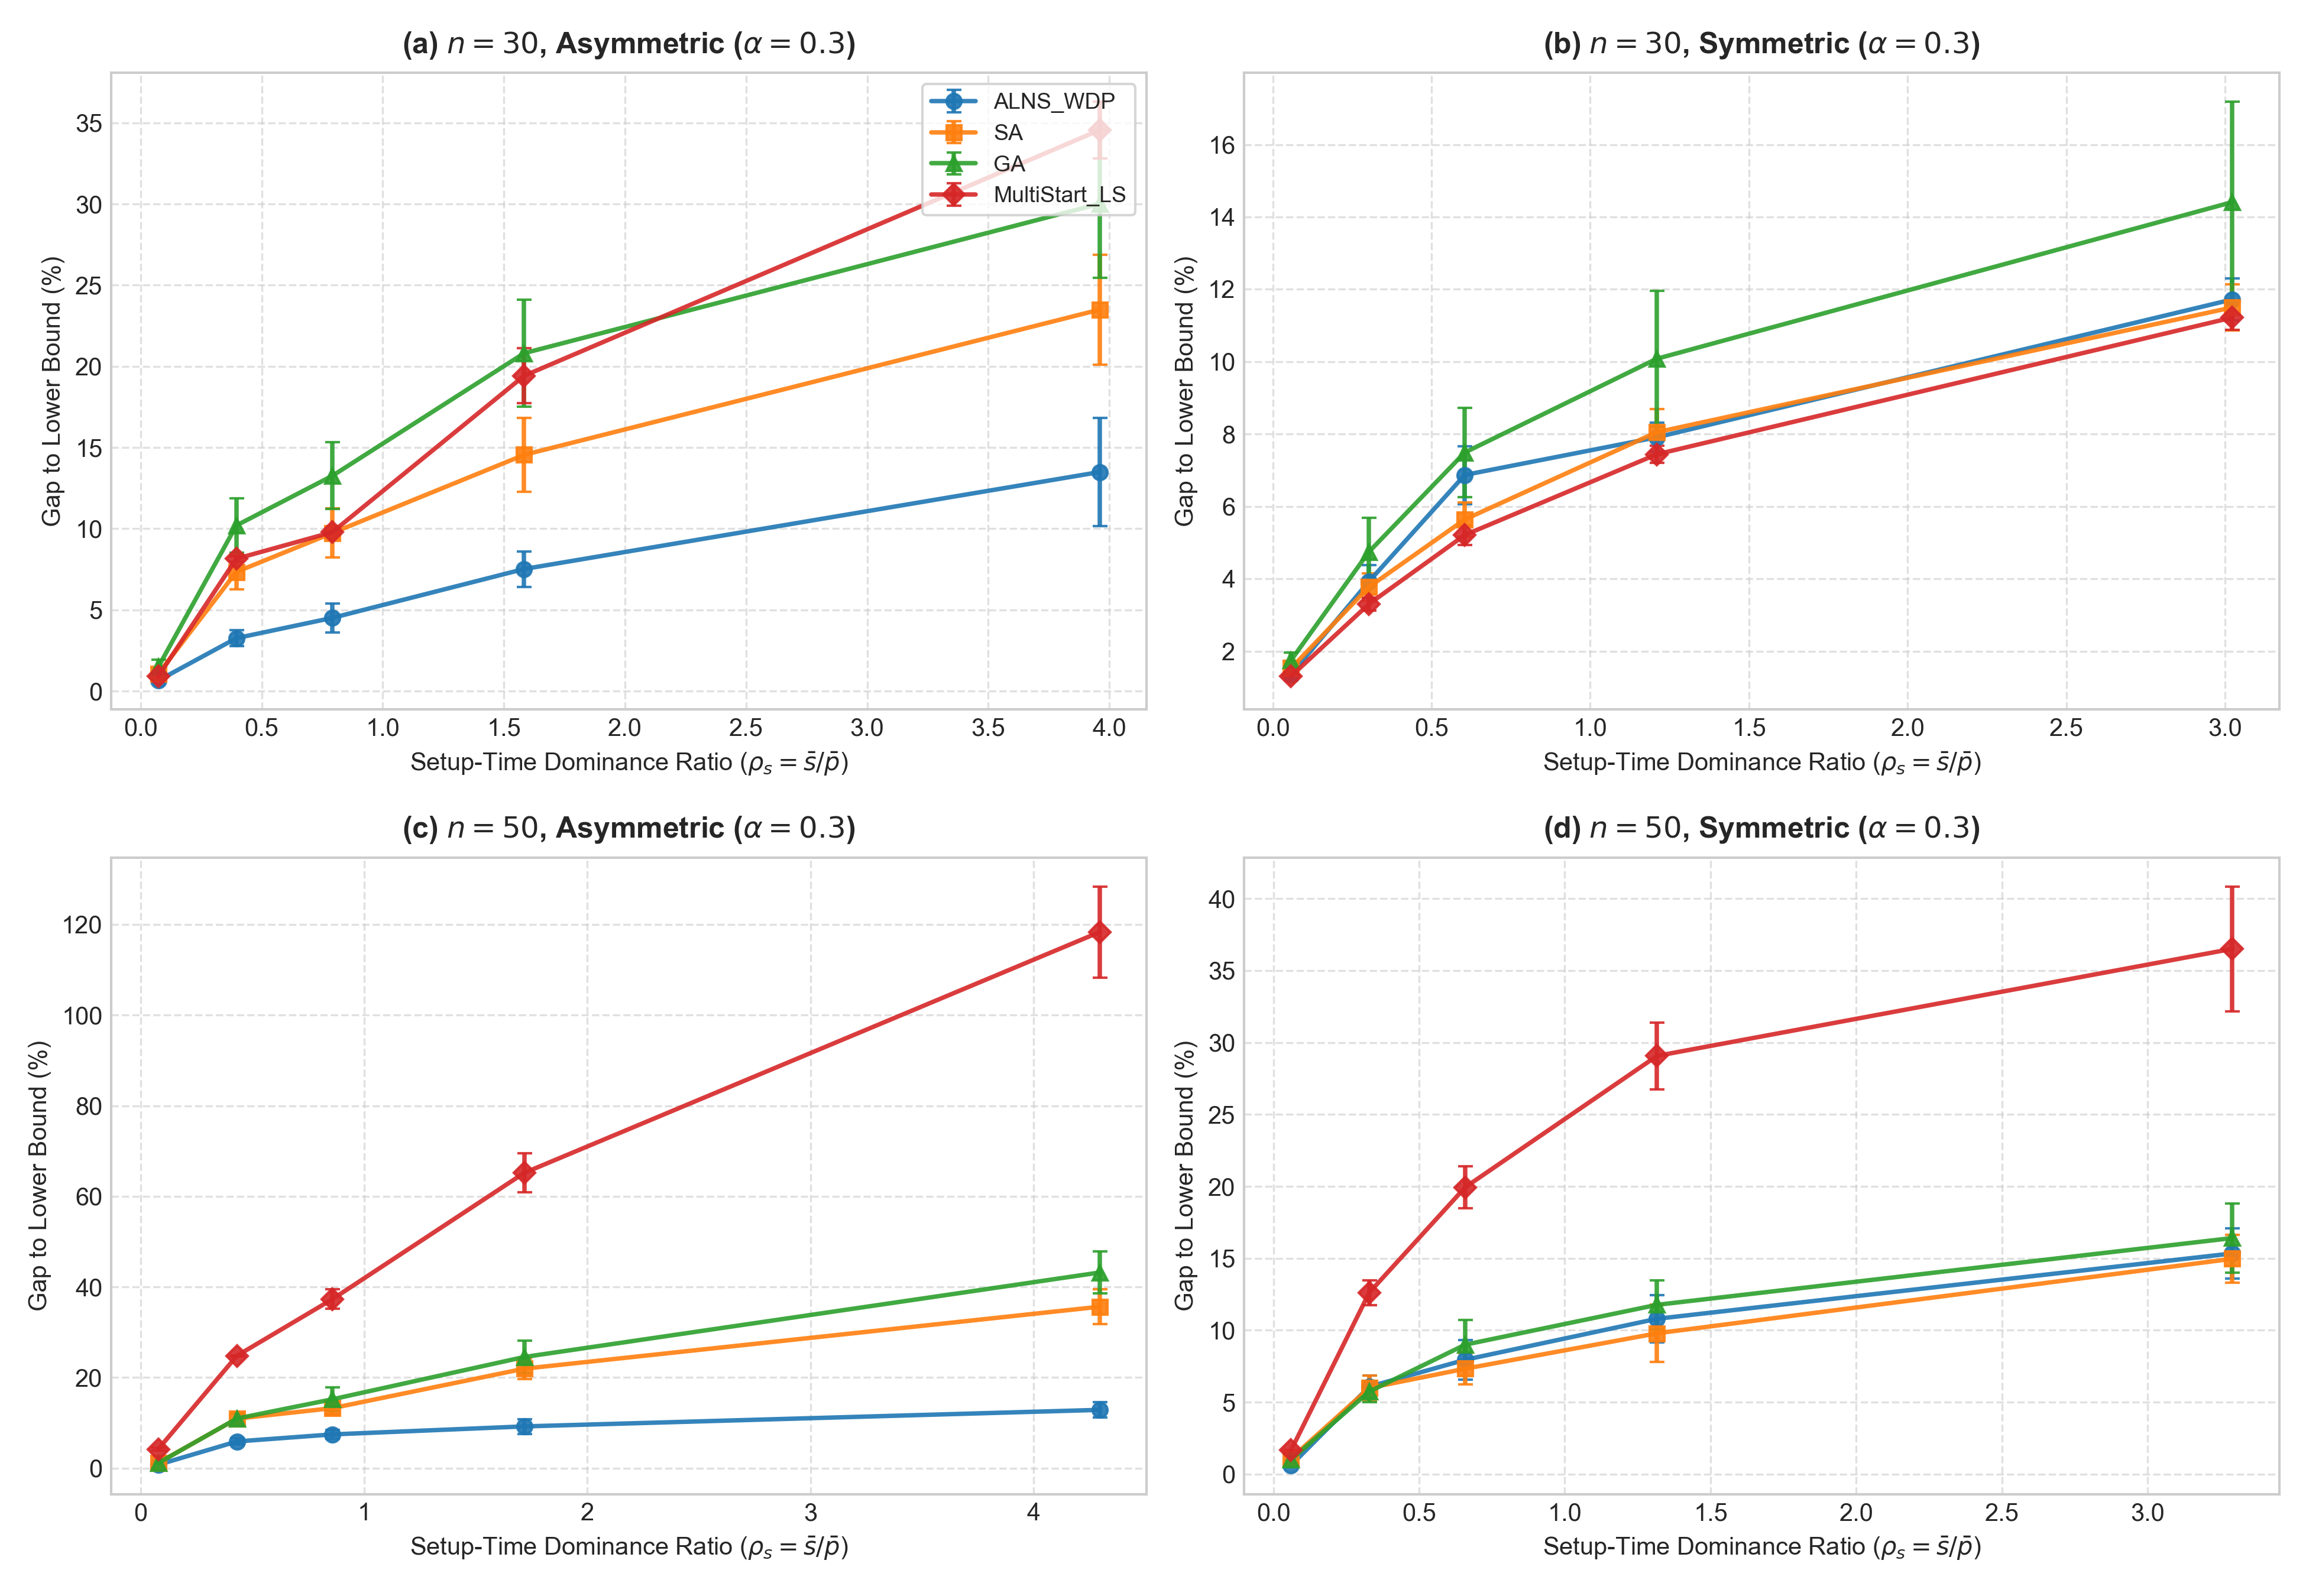
\includegraphics[width=\columnwidth]{figures/fig8_sensitivity_rho.png}
\caption{Controlled setup-time dominance sensitivity: Mean gap to valid lower bound (\%) vs. ratio $\rho_s = \bar{s}/\bar{p}$ across four base instances under matched nominal wall-clock budgets (30 seeds per cell).}
\label{fig:sensitivity_rho}
\end{figure}

\textbf{Statistical Analysis across Dual Hypothesis Families}: We define two distinct inferential families across the 60 pairwise comparisons:
\begin{enumerate}
    \item \textbf{Exploratory Family} ($m=3$ per configuration): Step-down Holm correction within each individual $(base, \beta)$ setting.
    \item \textbf{Confirmatory Family} ($m=60$ global): Global Holm-Bonferroni correction across the entire experimental suite.
\end{enumerate}

Key empirical findings:
\begin{itemize}
    \item \textbf{Asymmetric Dominance of ALNS-WDP}: On asymmetric setups, ALNS-WDP sweeps 10 out of 10 pairwise comparisons against SA, GA, and MultiStart\_LS under \textit{both} exploratory and global corrections (all 10 global Holm $p < 0.0001$). As setup dominance increases from $\rho_s \approx 0.08$ to $\rho_s \approx 4.30$, ALNS-WDP's makespan advantage over SA expands from $-0.41\%$ to $-16.78\%$ on $n=50$, and from $-0.41\%$ to $-8.10\%$ on $n=30$. MultiStart\_LS degrades severely on asymmetric setups as $\rho_s$ increases (gap expands to 118.30\% on $n=50$).
    \item \textbf{Symmetric Competitiveness of 2-Opt}: On symmetric setups, MultiStart\_LS and SA outperform ALNS-WDP at moderate-to-high setup ratios. On \texttt{n30\_a30\_sym} at $\beta=1.0$, MultiStart\_LS achieves 28 wins, 1 tie, and 1 loss against ALNS-WDP (global Holm $p < 0.0001$), while SA achieves 27 wins, 0 ties, and 3 losses (global Holm $p < 0.0001$).
    \item \textbf{Reassessment on Large Symmetric Instances}: Under exploratory correction ($m=3$), SA appeared significantly superior to ALNS-WDP on \texttt{n50\_a30\_sym} at $\beta=2.0$ (raw $p = 0.0300$, exploratory Holm $p = 0.0435$). However, under the confirmatory global family ($m=60$), this comparison yields global Holm $p = 0.3295$, failing to achieve statistical significance. Thus, on $n=50$ symmetric setups, differences between ALNS-WDP and SA remain inconclusive.
\end{itemize}

\section{Limitations and Threats to Validity}
\label{sec:limitations}

\begin{enumerate}
    \item \textbf{Single Instance at $n=200$}: The scalability evaluation at $n=200$ is based on a single instance (\texttt{n200\_a30\_asym\_s21003}). Multi-instance distributions were tested for $n \le 100$.
    \item \textbf{Exploratory Topology Analysis}: The 20-instance benchmark grid contains one instance per $(n, \alpha, \text{topology})$ cell. While the controlled setup-dominance experiment corroborated the split on 4 base instances, broader generalizability across arbitrary arrival patterns requires qualification.
    \item \textbf{2-Opt Reversal Advantage as a Hypothesis}: The superior performance of 2-opt descent on symmetric Euclidean setups is an architectural hypothesis—namely, that segment reversals $\pi(i \dots j) \to \pi(j \dots i)$ untangle Euclidean crossings without changing internal transition costs ($s_{uv} = s_{vu}$)—supported by empirical convergence, rather than a proven causal theorem.
    \item \textbf{Bi-Objective DP Scope}: Window-DP optimizes makespan only, explaining why NSGA-II attains higher Hypervolume.
    \item \textbf{Ablation Runtime Overhead}: Due to Python interpreter overhead during operator selection, full ALNS variants ran up to 1.15x longer than \texttt{WindowDP\_FinalPolishOnly} on small instances.
    \item \textbf{Negative Finding on Adaptive Weights}: Bandit operator adaptation showed no statistically significant benefit over static weights ($p = 1.000$).
\end{enumerate}

\section{Conclusion}
\label{sec:conclusion}

This investigation analyzed single-machine scheduling from its polynomial base case ($1 \mid\mid C_{\max}$) to its strongly NP-hard generalization ($1 \mid r_j, s_{ij} \mid C_{\max}$). We proposed and evaluated ALNS-WDP, a hybrid metaheuristic combining Adaptive Large Neighborhood Search with exact sliding-window Held-Karp dynamic programming. Empirical benchmarking across 20 instances up to $n=200$ demonstrated that ALNS-WDP achieves a lower mean gap to valid lower bound (5.47\%) than SA (6.65\%), GA (7.70\%), and MultiStart\_LS (14.89\%), with improvements statistically significant only against GA (Holm $p = 0.0146$) and not significant against SA or MultiStart\_LS ($p = 0.1281$). Controlled setup-dominance experiments demonstrated that ALNS-WDP's advantage expands dramatically on asymmetric setups as setup costs dominate (Holm $p < 0.0001$), while reversal-based local search appears competitive on symmetric Euclidean setups, although the underlying mechanism remains a hypothesis requiring further investigation.

\appendix
\section{Claim-to-Evidence Traceability Matrix}
Table~\ref{tab:traceability} maps every empirical claim in this report to its exact source file in \texttt{results/} and the producing script.

\begin{table*}[htbp]
\centering
\small
\caption{Traceability Matrix: Report Claims to Results Files.}
\label{tab:traceability}
\begin{tabularx}{\textwidth}{p{5.5cm}p{6.0cm}p{4.5cm}}
\toprule
\textbf{Claim in Report} & \textbf{Evidence File} & \textbf{Generating Script} \\
\midrule
20 benchmark instances, 30 seeds & \texttt{results/single\_objective\_benchmarks.csv} & \texttt{src/experiments.py} \\
ALNS-WDP mean gap to LB = 5.47\% & \texttt{results/single\_objective\_benchmarks.csv} & \texttt{tools/rerun\_budget\_enforced.py} \\
ALNS-WDP gap to opt (n$\le$20) = 0.45\% & \texttt{results/single\_objective\_benchmarks.csv} & \texttt{tools/rerun\_budget\_enforced.py} \\
Competitor gaps: SA 6.65\%, GA 7.70\% & \texttt{results/single\_objective\_benchmarks.csv} & \texttt{src/experiments.py} \\
MultiStart\_LS gap = 14.89\%, rt = 1.42s & \texttt{results/single\_objective\_benchmarks.csv} & \texttt{tools/rerun\_multistart\_ls.py} \\
Friedman test $\chi^2=10.50, p=0.0148$ & \texttt{results/friedman\_ranks.csv} & \texttt{src/stats.py} \\
Wilcoxon Holm p: GA 0.0146, SA 0.1281 & \texttt{results/metaheuristic\_statistical\_tests.csv} & \texttt{src/stats.py} \\
Ablation: 600 runs, full gap = 5.06\% & \texttt{results/ablation\_results.csv} & \texttt{tools/rerun\_budget\_enforced.py} \\
Sensitivity to window size $k$ & \texttt{results/sensitivity\_k.csv} & \texttt{src/experiments.py} \\
Bi-objective HV and IGD metrics & \texttt{results/biobjective\_metrics.csv} & \texttt{tools/rerun\_budget\_enforced.py} \\
Stratified topology comparison & \texttt{results/stratified\_topology\_comparison.csv} & \texttt{src/stats.py} \\
Bi-objective Wilcoxon + Holm tests & \texttt{results/biobjective\_statistical\_tests.csv} & \texttt{src/stats.py} \\
Controlled setup dominance (2400 runs) & \texttt{results/sensitivity\_rho.csv} & \texttt{tools/run\_rho\_sensitivity.py} \\
Controlled setup dominance summary & \texttt{results/sensitivity\_rho\_summary.csv} & \texttt{tools/run\_rho\_sensitivity.py} \\
Controlled setup dominance stats & \texttt{results/sensitivity\_rho\_statistical\_tests.csv} & \texttt{tools/run\_rho\_sensitivity.py} \\
Setup dominance figure & \texttt{figures/fig8\_sensitivity\_rho.png} & \texttt{tools/run\_rho\_sensitivity.py} \\
\bottomrule
\end{tabularx}
\end{table*}

\begin{thebibliography}{99}
\bibitem{pinedo2016scheduling} M.~L. Pinedo, \emph{Scheduling: Theory, Algorithms, and Systems}, 5th~ed. Springer, New York, 2016.
\bibitem{graham1979optimization} R.~L. Graham, E.~L. Lawler, J.~K. Lenstra, and A.~H.~G. Rinnooy~Kan, ``Optimization and approximation in deterministic sequencing and scheduling: a survey,'' \emph{Annals of Discrete Mathematics}, vol.~5, pp. 287--326, 1979.
\bibitem{garey1979computers} M.~R. Garey and D.~S. Johnson, \emph{Computers and Intractability: A Guide to the Theory of NP-Completeness}. W. H. Freeman and Company, San Francisco, 1979.
\bibitem{ropke2006adaptive} S.~Ropke and D.~Pisinger, ``An adaptive large neighborhood search heuristic for the pickup and delivery problem with time windows,'' \emph{Transportation Science}, vol.~40, no.~4, pp. 455--472, 2006, doi: 10.1287/trsc.1050.0135.
\bibitem{pisinger2010large} D.~Pisinger and S.~Ropke, ``Large neighborhood search,'' in \emph{Handbook of Metaheuristics}, M.~Gendreau and J.-Y.~Potvin, Eds. Springer, Boston, MA, 2010, pp. 399--419, doi: 10.1007/978-1-4419-1665-5\_13.
\bibitem{shaw1998using} P.~Shaw, ``Using constraint programming and local search methods to solve vehicle routing problems,'' in \emph{Principles and Practice of Constraint Programming (CP98)}, LNCS 1520:417--431. Springer, 1998, doi: 10.1007/3-540-49481-2\_30.
\bibitem{held1962dynamic} M.~Held and R.~M. Karp, ``A dynamic programming approach to sequencing problems,'' \emph{Journal of the Society for Industrial and Applied Mathematics}, vol.~10, no.~1, pp. 196--210, 1962, doi: 10.1137/0110015.
\bibitem{balas2001linear} E.~Balas and N.~Simonetti, ``Linear time dynamic-programming algorithms for new classes of restricted TSPs: A computational study,'' \emph{INFORMS Journal on Computing}, vol.~13, no.~1, pp.~56--75, 2001, doi: 10.1287/ijoc.13.1.56.9748.
\bibitem{congram2002iterated} R.~K. Congram, C.~N. Potts, and S.~L. van de Velde, ``An iterated dynasearch algorithm for the single-machine total weighted tardiness scheduling problem,'' \emph{INFORMS Journal on Computing}, vol.~14, no.~1, pp.~52--67, 2002, doi: 10.1287/ijoc.14.1.52.7712
\bibitem{sourd2006dynasearch} F.~Sourd, ``Dynasearch for the earliness-tardiness scheduling problem with release dates and setup constraints,'' \emph{Operations Research Letters}, vol.~34, no.~5, pp. 591--598, 2006, doi: 10.1016/j.orl.2005.06.005.
\bibitem{allahverdi2015third} A.~Allahverdi, ``The third comprehensive review on scheduling problems with setup times/costs,'' \emph{European Journal of Operational Research}, vol.~246, no.~2, pp. 345--378, 2015, doi: 10.1016/j.ejor.2015.04.004.
\bibitem{archetti2014survey} C.~Archetti and M.~G. Speranza, ``A survey on matheuristics for routing problems,'' \emph{EURO Journal on Computational Optimization}, vol.~2, no.~4, pp. 223--246, 2014, doi: 10.1007/s13675-014-0030-7.
\bibitem{deb2002fast} K.~Deb, A.~Pratap, S.~Agarwal, and T.~Meyarivan, ``A fast and elitist multiobjective genetic algorithm: NSGA-II,'' \emph{IEEE Transactions on Evolutionary Computation}, vol.~6, no.~2, pp. 182--197, 2002, doi: 10.1109/4235.996017.
\bibitem{kuhn1955hungarian} H.~W. Kuhn, ``The Hungarian method for the assignment problem,'' \emph{Naval Research Logistics Quarterly}, vol.~2, no.~1--2, pp. 83--97, 1955, doi: 10.1002/nav.3800020109.
\end{thebibliography}

\end{document}
